\chapter{Impulse and Momentum}
	\section{Momentum} \label{momentum} \index{Momentum} \index{Momentum, Linear}
	Linear momentum is defined by the following equation:
	\begin{mdframed}[backgroundcolor=orange!20!white]
		\begin{equation}
		\vec{p} \equiv m \vec{v} 
		\label{eqn:momentum}
		\end{equation}
	\end{mdframed}
	 where $\vec{p}$ is momentum, $m$ is mass, and $\vec{v} $ is velocity.  Determining an object's momentum can be extremely useful in solving problems involving collisions or explosions.  
	 
	 \begin{mdframed}[backgroundcolor=blue!10!white]
	 	\begin{center}
	 		
	 		
	 		\textbf{Example \thesection.1}	
	 	\end{center}
	 	
	 	\textbf{Problem: } A 1400 kg bus is traveling at 12 m/s.  What is its momentum? 
	 	\vspace{0.1in}
	 	
	 	\textbf{Solution:} 
	 	Begin by drawing a diagram and identifying variables:
	 		 \vspace{0.2in}
	 	
	 	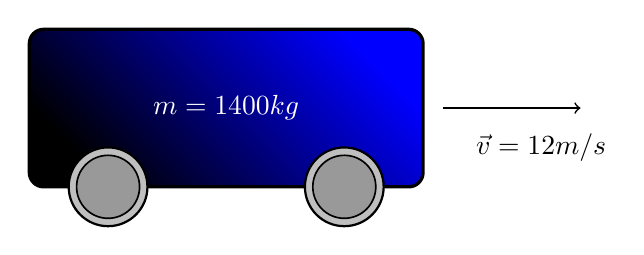
\begin{tikzpicture}
	 		\shade[top color=blue, bottom color=black, shading angle={-45}]
	 		[draw=black,fill=red!20,rounded corners=1.2ex,very thick] (1.5,.5) rectangle (6.5,2.5);
	 		\draw[draw=black,fill=gray!50,thick] (2.5,.5) circle (.5);
	 		\draw[draw=black,fill=gray!50,thick] (5.5,.5) circle (.5);    
	 		\draw[draw=black,fill=gray!80,semithick] (2.5,.5) circle (.4);
	 		\draw[draw=black,fill=gray!80,semithick] (5.5,.5) circle (.4);
	 		
	 		\draw[->,semithick] (6.75,1.5) -- (8.5,1.5);
	 		\draw (8,1) node {$\vec{v} = 12 \si{m/s}$};
	 		\draw (4,1.5) node[text=white] {$m = 1400 \si{kg}$};
	 	\end{tikzpicture}
	 	
	 	Using equation \ref{eqn:momentum}, we see:
	 	\begin{equation*}
	 	\vec{p} = m \vec{v} = 1400 kg \times 12 \frac{m}{s} = \boxed{16800 \frac{kg\cdot m}{s}}
	 	\end{equation*}
	 	
	 \end{mdframed}
	 \vspace{0.1in}
	 You may notice that the units for momentum are $\frac{kg \cdot m} {s}$.  This is read as ``kilogram meters per second,'' and there is no special name for this unit.  
	 
	 
	\section{Impulse} \label{impulse} \index{Impulse}
		When a force is applied to an object for a certain amount of time, an \textit{impulse} is delivered to that object.  Impulse is defined by the following equation:
	\begin{mdframed}[backgroundcolor=orange!20!white]
		\begin{equation}
		\vec{J} \equiv \vec{F} t 
		\label{eqn:Impulse}
		\end{equation}
	\end{mdframed}
	where $\vec{J}$ is impulse, $\vec{F}$ is force, and $t $ is time.  The units for impulse are $\si{N\cdot s}$, which are equivalent to $ \si{\frac{kg \cdot m}{s}}$.
	
	
	
	
	\section{The Impulse-Momentum Theorem}
	
	Just as work causes an object's energy to change, impulse causes an object's momentum to change:
	
		\begin{mdframed}[backgroundcolor=orange!20!white]
		\begin{equation}
		\vec{J} = \Delta \vec{p} 
		\label{eqn:ImpulseMomentumTheorum}
		\end{equation}
	\end{mdframed}
	
	
	
	
	\section{The Law of Conservation of Momentum}
	\index{Law of Conservation of Momentum}
	\index{Momentum, Law of Conservation of}
	
	The Law of Conservation of Momentum states that momentum cannot be created or destroyed.  Thus, the total momentum a system has in its initial state, plus any changes in momentum from outside the system (accounted for as impulse) must be equal to the total momentum the system has in its final state.
	
	
	\begin{mdframed}[backgroundcolor=orange!20!white]
		\begin{equation}
			\vec{p_i} + \vec{J} = \vec{p_f}
			\label{eqn:ConservationofMomentum}
		\end{equation}
	\end{mdframed}
	

	 \begin{mdframed}[backgroundcolor=blue!10!white]
	\begin{center}
	\textbf{Example \thesection.1}	
	\end{center}
	
	\textbf{Problem: } A 1000 kg car is traveling to the right at 12 m/s.  It collides head-on with an 800 kg car traveling to the left at 8 m/s.  The two cars get stuck together.  What is the velocity of the wreckage immediately after the collision?
	
	\vspace{0.1in}
	
	\textbf{Solution:} 
	Begin by drawing a diagram and identifying variables:
	
	
	\begin{equation*}
		\vec{p} = m \vec{v} = 1400 kg \times 12 \frac{m}{s} = 16800 \frac{kg\cdot m}{s}
	\end{equation*}
	
\end{mdframed}
\vspace{0.1in}

	


